\section{実験結果}
\label{sec:results}
\subsection{Lorenz96における構造回復}
表\ref{tab:lorenz-results}に構造回復の結果を示す。\(T=500\)ではGSE-VARが全5系列で60真辺を過不足なく選択した。

\begin{table}[H]
\centering\small
\caption{Lorenz96の構造回復。5系列の平均\(\pm\)標本標準偏差。PR面積は観測点間の台形積分、F1と辺数は独立な予備探索で選んだ設定の値である。自己辺を除外し、各条件・指標の最大平均値を太字とした。}
\label{tab:lorenz-results}
\setlength{\tabcolsep}{4pt}
\begin{tabular}{rlrrr}
\toprule
\(T\)&手法&AUPRC&F1&辺数\\
\midrule
250&GSE-VAR&\(\mathbf{0.9998}\pm0.0004\)&\(\mathbf{0.997}\pm0.007\)&60.4\\
&NGC&\(0.5233\pm0.0589\)&\(0.454\pm0.053\)&44.0\\
&GVAR&\(0.8217\pm0.0689\)&\(0.616\pm0.094\)&35.6\\
&線形VAR&\(0.4103\pm0.0913\)&\(0.226\pm0.125\)&15.4\\
\midrule
500&GSE-VAR&\(\mathbf{1.0000}\pm0.0000\)&\(\mathbf{1.000}\pm0.000\)&60.0\\
&NGC&\(0.7434\pm0.0336\)&\(0.628\pm0.070\)&34.4\\
&GVAR&\(0.9941\pm0.0044\)&\(0.866\pm0.044\)&48.2\\
&線形VAR&\(0.6430\pm0.0622\)&\(0.478\pm0.053\)&26.8\\
\bottomrule
\end{tabular}
\end{table}

図\ref{fig:lorenz-paths}では、GSE-VARが高い適合率を保ちながら真辺を選択している。\(T=250\)の平均AUPRCは\(0.9998\)、\(T=500\)では\(1.0000\)となった。

\begin{figure}[H]
\centering
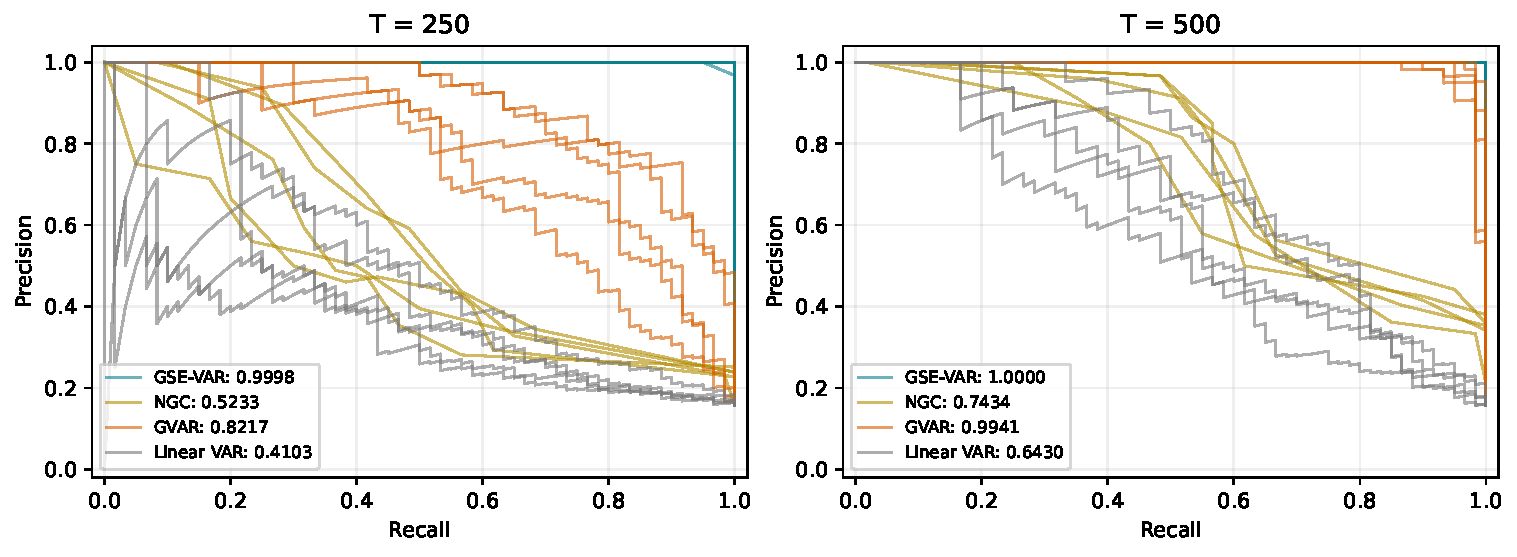
\includegraphics[width=\linewidth]{figures/lorenz_lambda_paths.pdf}
\caption{Lorenz96のPR曲線。各条件の5系列を重ねた。GSE-VARとNGCは正則化10候補で選択された辺、GVARと線形VARはそれぞれ係数強度と負の\(p\)値に対する閾値を変えて求める。線は観測点間を結び、凡例は平均AUPRCを示す。}
\label{fig:lorenz-paths}
\end{figure}

図\ref{fig:lorenz-structures}で選択頻度を示す。GVARの\(T=500\)ではAUPRCが高くても採用グラフには見落としが残り、順位評価と固定グラフの回復は一致しない。

\begin{figure}[!htbp]
\centering
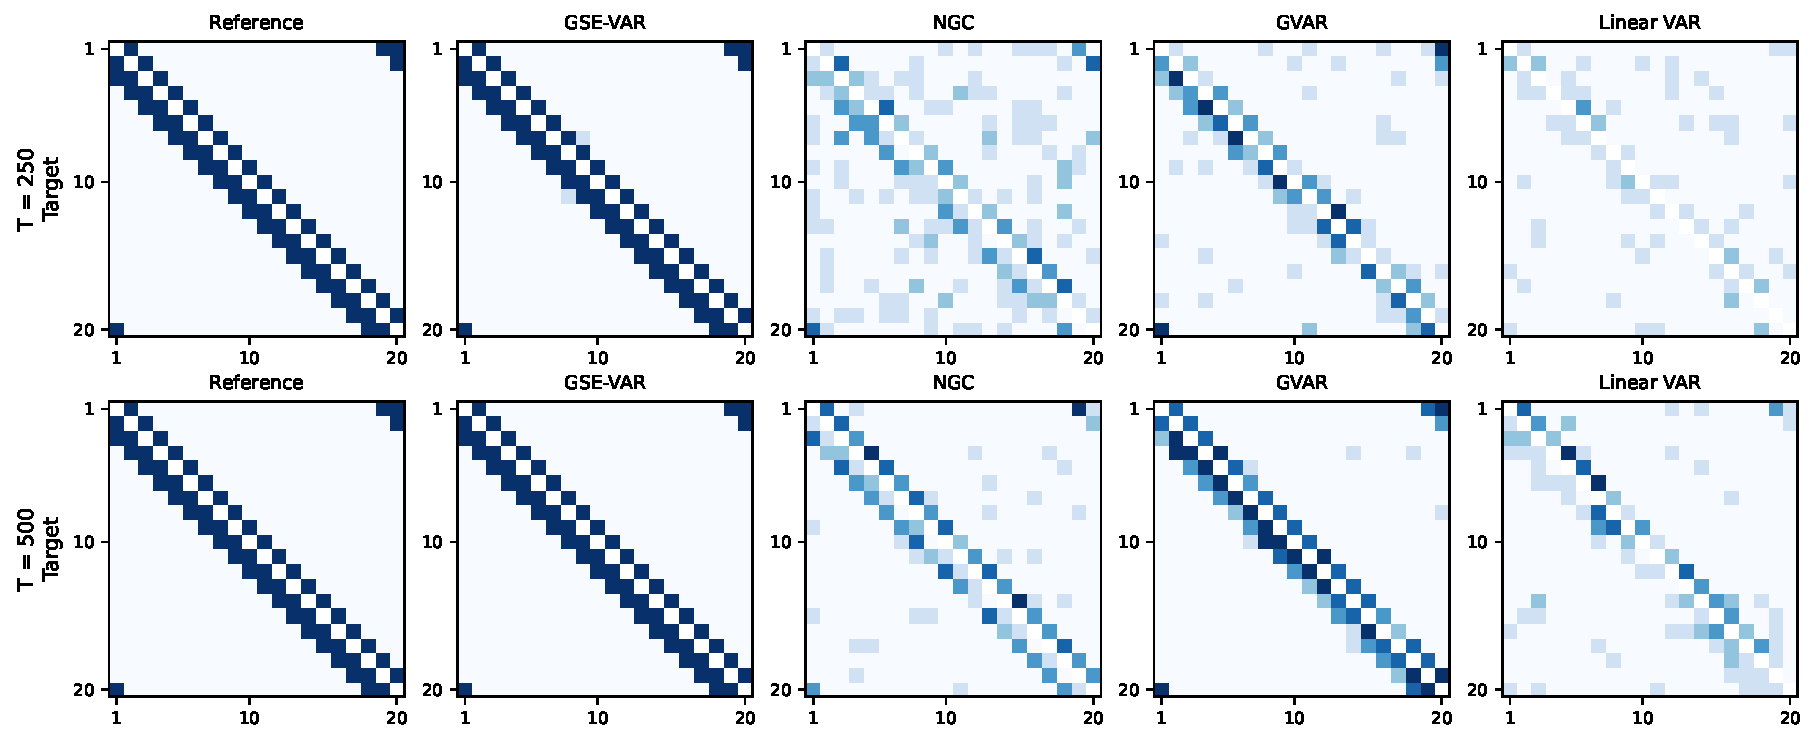
\includegraphics[width=\linewidth]{figures/lorenz_structures.pdf}
\caption{Lorenz96の参照構造と各手法の辺選択頻度。行は予測対象、列は入力系列であり、色は5回の実験で辺が選択された割合を示す。上段は\(T=250\)、下段は\(T=500\)。自己辺は灰色とした。}
\label{fig:lorenz-structures}
\end{figure}

\subsection{線形VAR過程における符号回復}
表\ref{tab:linear-results}では、両系列長とも線形VARの平均符号BAが最も高い。GSE-VARは\(T=250,500\)でそれぞれ\(0.900\)、\(0.975\)となり、GVARを上回った。

\begin{table}[H]
\centering\small
\caption{線形VARの符号回復。10系列の平均\(\pm\)標本標準偏差。正・負のBAはそれぞれの符号を陽性として算出し、その平均を主指標とする。各条件・指標の最大平均値を太字とした。}
\label{tab:linear-results}
\setlength{\tabcolsep}{4pt}
\begin{tabular}{rlrrr}
\toprule
\(T\)&手法&\(\mathrm{BA}_{pos}\)&\(\mathrm{BA}_{neg}\)&平均符号BA\\
\midrule
250&GSE-VAR&\(0.908\pm0.169\)&\(0.892\pm0.167\)&\(0.900\pm0.129\)\\
&GVAR&\(0.883\pm0.172\)&\(0.877\pm0.178\)&\(0.880\pm0.157\)\\
&線形VAR&\(\mathbf{0.995}\pm0.014\)&\(\mathbf{0.990}\pm0.021\)&\(\mathbf{0.993}\pm0.012\)\\
\midrule
500&GSE-VAR&\(0.975\pm0.079\)&\(0.975\pm0.079\)&\(0.975\pm0.053\)\\
&GVAR&\(0.895\pm0.172\)&\(0.912\pm0.178\)&\(0.903\pm0.140\)\\
&線形VAR&\(\mathbf{0.995}\pm0.014\)&\(\mathbf{0.990}\pm0.020\)&\(\mathbf{0.993}\pm0.011\)\\
\bottomrule
\end{tabular}
\end{table}

図\ref{fig:linear-coefficients}に全12非自己係数を示す。GSE-VARでは符号が一致しても係数が大きく変動する場合がある。

\begin{figure}[H]
\centering
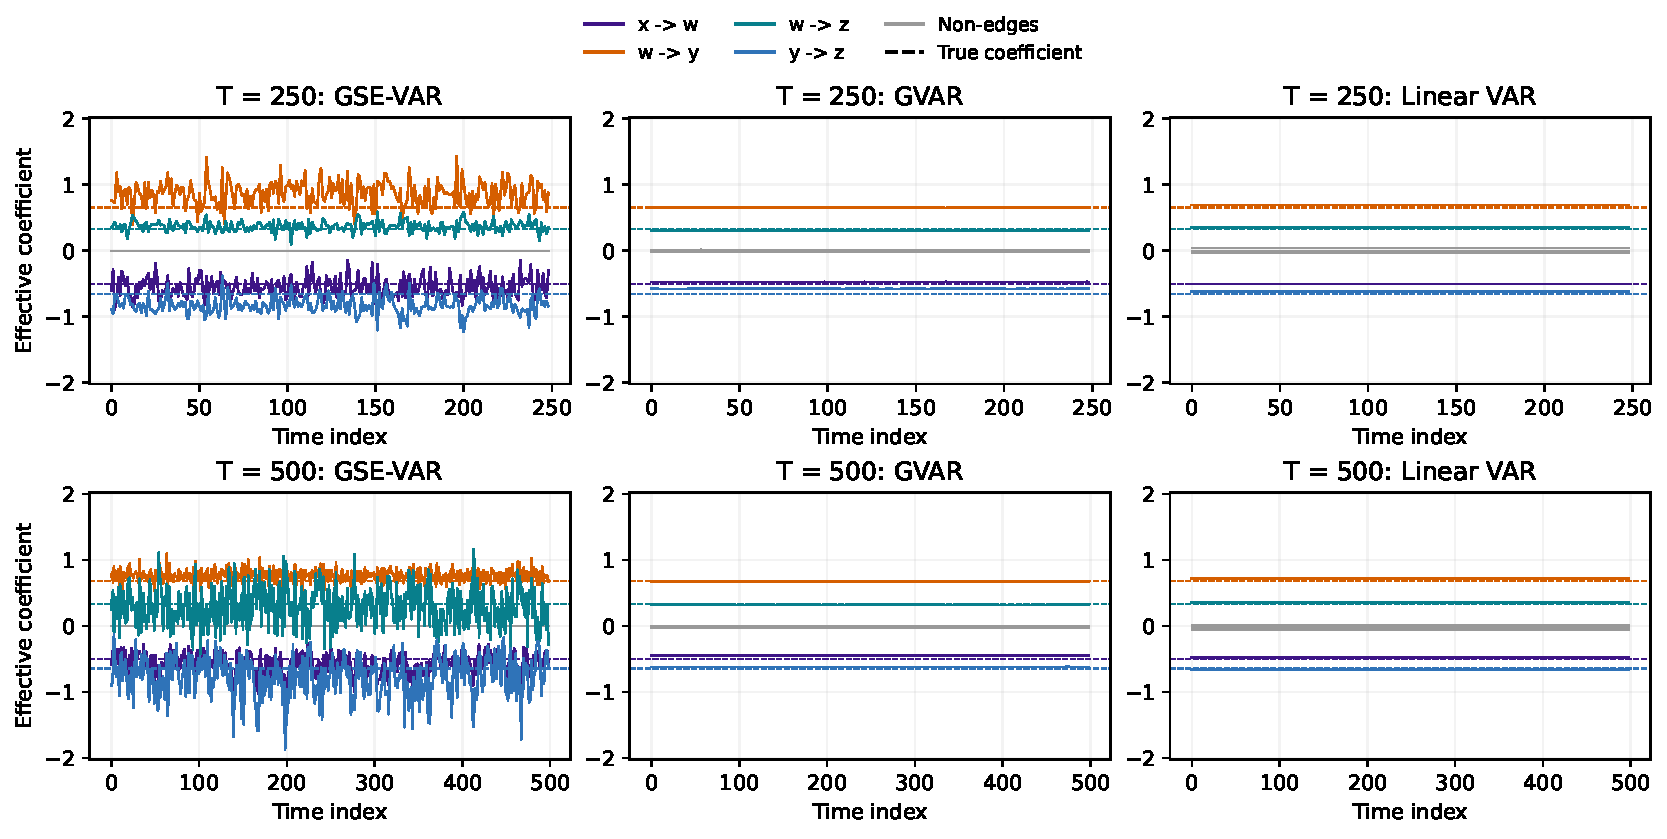
\includegraphics[width=.94\linewidth]{figures/linear_coefficients.pdf}
\caption{線形VARの全12非自己係数。上段は\(T=250\)、下段は\(T=500\)の第1系列。左からGSE-VAR、GVAR、線形VAR。色付き実線は4真辺、灰色実線は8非辺、破線は標準化後の真値を示す。全6パネルの縦軸を共通とし、平滑化や値の切り捨ては行っていない。}
\label{fig:linear-coefficients}
\end{figure}
